\providecommand{\main}{../..}
\documentclass[\main/dresen_thesis.tex]{subfiles}

\begin{document}
\chapter{Loosely-packed nanostructures}\label{ch:looselyPackedNS}
Magnetic nanospheres can nowadays be routinely synthesized from a large choice of materials \cite{Gubin_2005_Magne}.
Magnetite ($\ch{Fe3O4}$) is a common choice for the study of nanomagnetism as it shows strong ferromagnetism and is widely available.
Due to this extensive research it is now possible to synthesize iron oxide nanoparticles that are highly tunable in size and shape \cite{Wetterskog_2014_Preci}.
In this work, two batches of iron oxide nanospheres in the size range of $11 \unit{nm}$ (IOS-11) and $7 \unit{nm}$ (IOS-7) are studied for their individual structural and magnetic properties.
Furthermore, loosely packed layers of the nanoparticles, created by spin coating the particles from dispersion on a substrate, are studied.
The magnetic properties of the nanostructure are compared to the individual nanoparticle properties and compared to model calculations to search for emergent effects arising from dipolar interparticle interaction.

\section{Spherical iron oxide nanoparticles}
Iron oxide nanoparticles were obtained from a collaboration with the group of Prof. Tremel from the inorganic chemistry department of the university of Mainz.
Briefly, they were prepared by following a popular synthesis route where first iron oleate is prepared from iron(III) chloride and then nanospheres are obtained by a controlled thermal decomposition of the oleate in a high boiling solvent (1-Octadecene).
A similar synthesis procedure is used in \refsec{ch:monolayers} for the preparation of cobalt iron oxide nanocubes and is explained in that section in more detail.

\begin{figure}[tb]
  \centering
  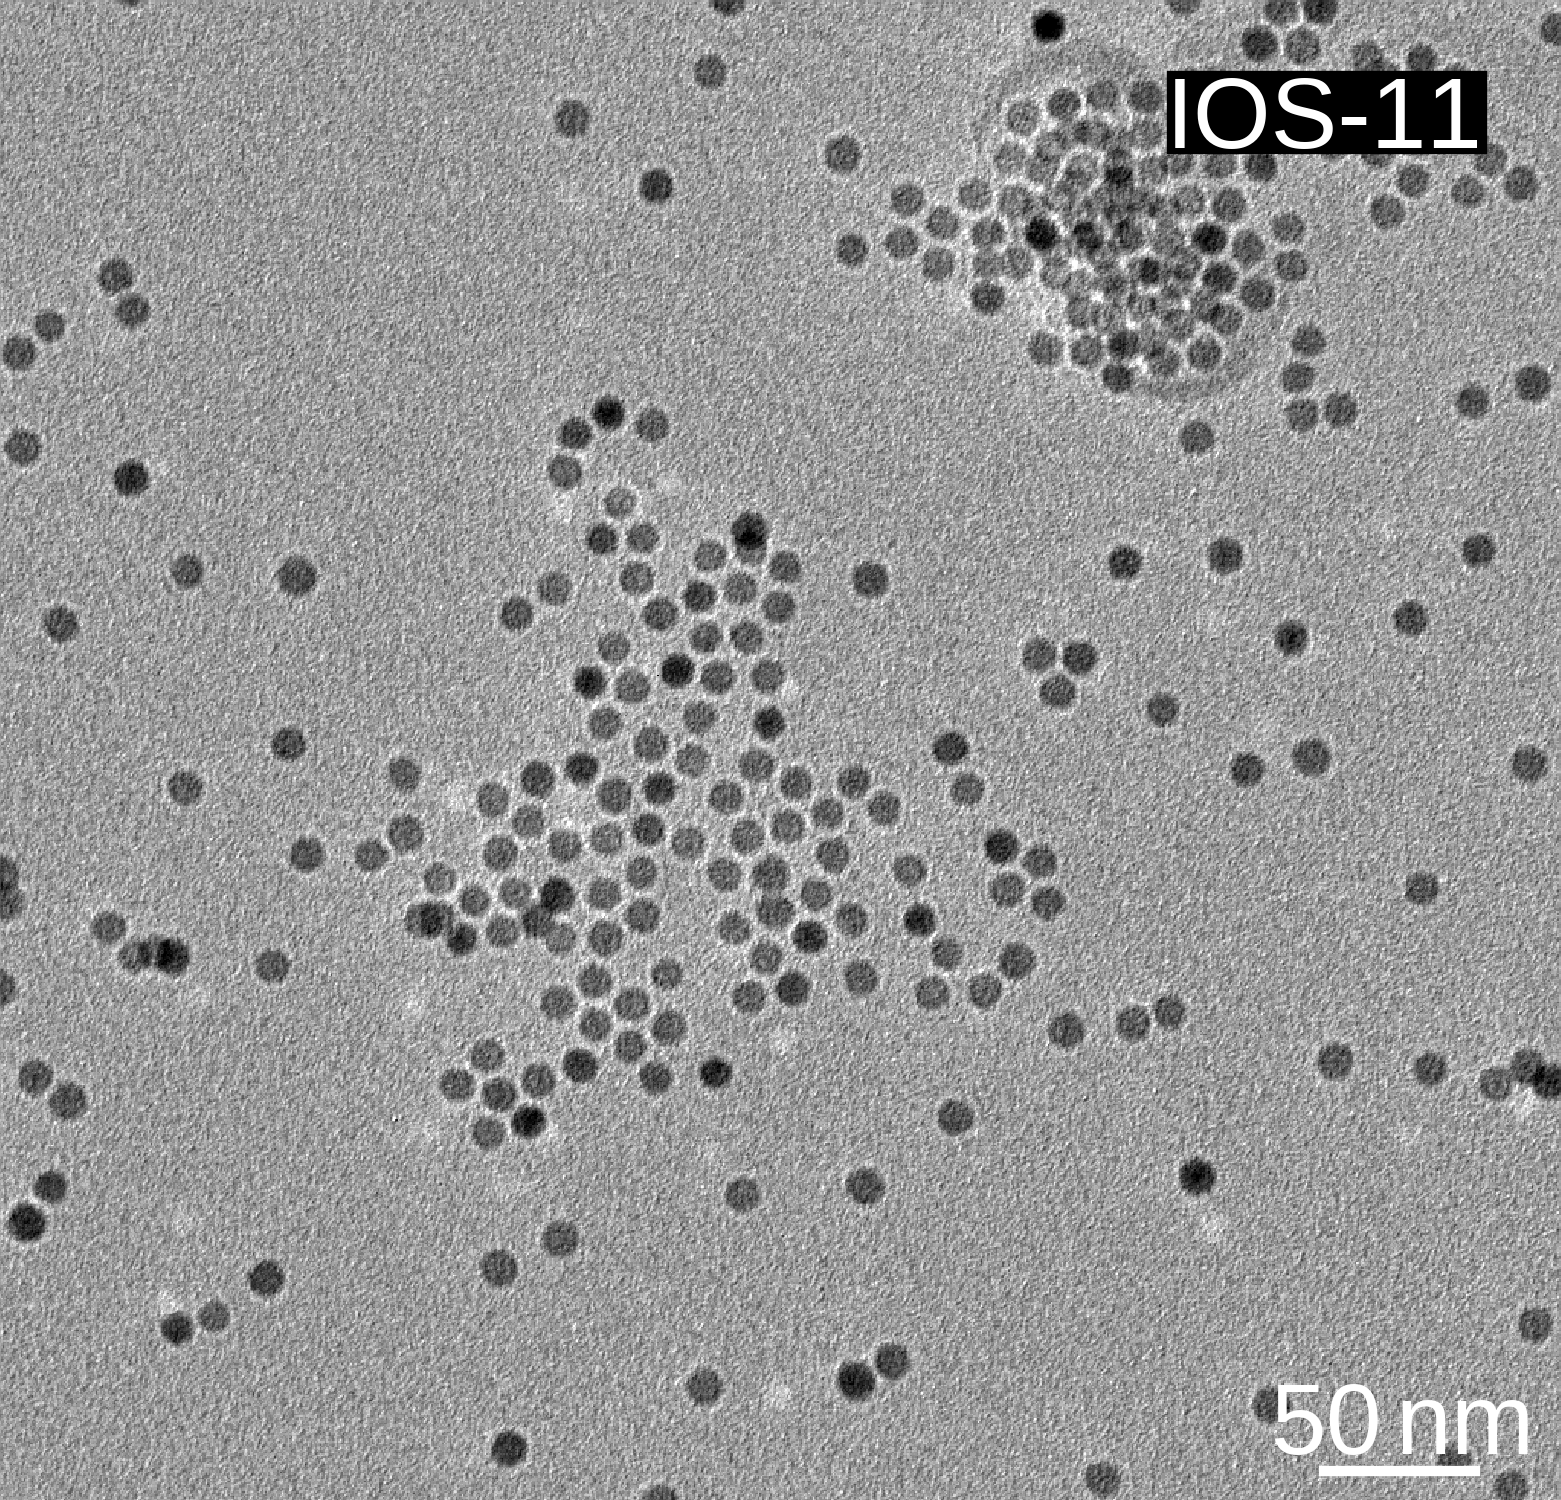
\includegraphics{looselyPackedNP_TEM_PMK18}
  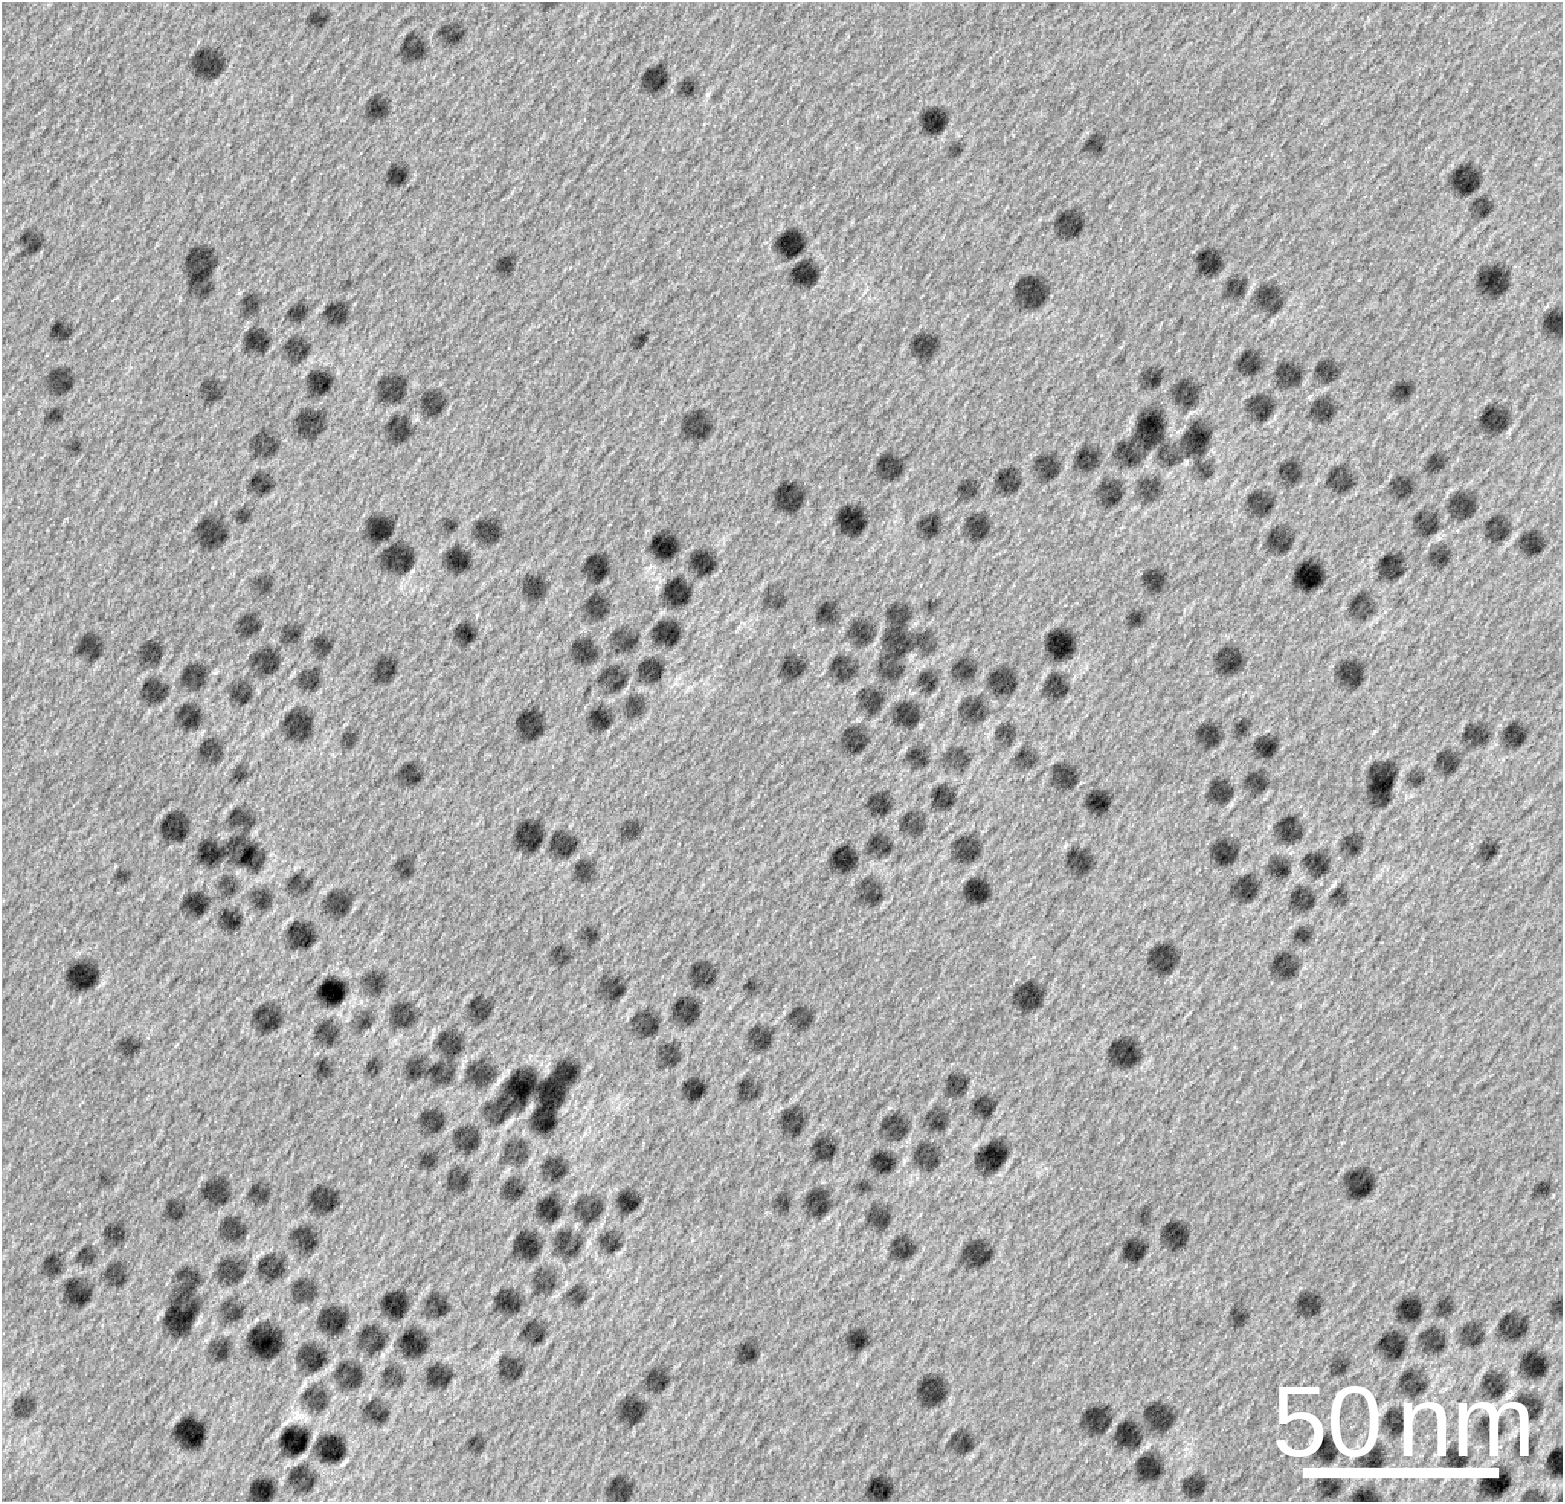
\includegraphics{looselyPackedNP_TEM_KWi338}
  \caption{\label{fig:looselyPackedNP:nanoparticle:tem}Transmission electron microscopy images of iron oxide nanospheres IOS-11 (left) and IOS-7 (right).}
\end{figure}

In a first step, the iron oxide nanospheres are characterized by transmission electron microscopy.
The measurements in \reffig{fig:looselyPackedNP:nanoparticle:tem} show the spherical shape of the nanoparticles.
By manually measuring the diameters of $\approx 200$ particles each, the probability density is estimated for both batches.
In \reffig{fig:looselyPackedNP:nanoparticle:temSizeDist}, the counted diameters are shown as histogram and both distributions are fit using the log-normal distribution
\begin{align}
  p(d; \mu, \sigma) \eq \frac{1}{\sqrt{2\pi} \sigma d} \exp \biggl( - \frac{\log(d) - \log(\mu)}{2 \sigma^2} \biggr),
\end{align}
where the parameters $\mu$ and $\sigma$ relate to the expectation value and standard deviation of the distribution via
\begin{align}
  E[d] \eq& \mu e^{\sigma^2/2} \approx \mu,\\
  Std[d] \eq& \mu e^{\sigma^2/2} \sqrt{e^{\sigma^2} - 1} \approx \mu \sigma,\\
\end{align}
with the approximations being valid for $\sigma^2 \ll 1$.
The log-normal distribution is generally used to model nanoparticle size distribution phenomenologically as it allows only for positive numbers.
As all size distributions are in the order of $10 \, \%$ in this work, it follows that the width parameter is $\sigma \approx \mathcal{O}(0.1)$ and with the approximations $\mu$ can be treated as the expectation value and $\sigma$ as the relative standard deviation.

The batch IOS-11 is well described by a single log-normal function. The second batch, however, has a broader size distribution with additionally smaller particles inside.
In this case a bimodal log-normal distribution is better suited
\begin{align}
  p(d) \eq N_1 p_1(d; \mu_1, \sigma_1) + N_2 p_2(d; \mu_2, \sigma_2),
\end{align}
with $N_1 + N_2 = 1$.
Here, the batch is described by being one part particles with a narrow size distribution and one part with a broad size distribution.
The estimated parameters for both samples are listed in \reftab{tab:looselyPackedNP:nanoparticle:temModel}.
\begin{figure}[tb]
    \centering
    \captionof{table}{\label{tab:looselyPackedNP:nanoparticle:temModel}Parameters estimated for the size distribution of IOS-11 and IOS-7 from fitting a (bimodal) log-normal size distribution.}
    \begin{minipage}{0.49\textwidth}
      \centering
      \begin{tabular}{ c | l | l }
          & IOS-11 & IOS-7 \\
        \hline
        $N_1$       & $1$                   & $0.7(1)$   \\
        $\mu_1$     & $10.95(5) \unit{nm}$  & $6.97(6) \unit{nm}$ \\
        $\sigma_1$  & $6.6(4) \unit{\%}$    & $11(1) \unit{\%}$ \\
        $N_2$       & 0                     & $0.3(1)$  \\
        $\mu_2$     & -                     & $6.0(6) \unit{nm}$ \\
        $\sigma_2$  & -                     & $29(4) \unit{\%}$ \\
        \hline
      \end{tabular}
    \end{minipage}
    \begin{minipage}{0.49\textwidth}
      \centering
      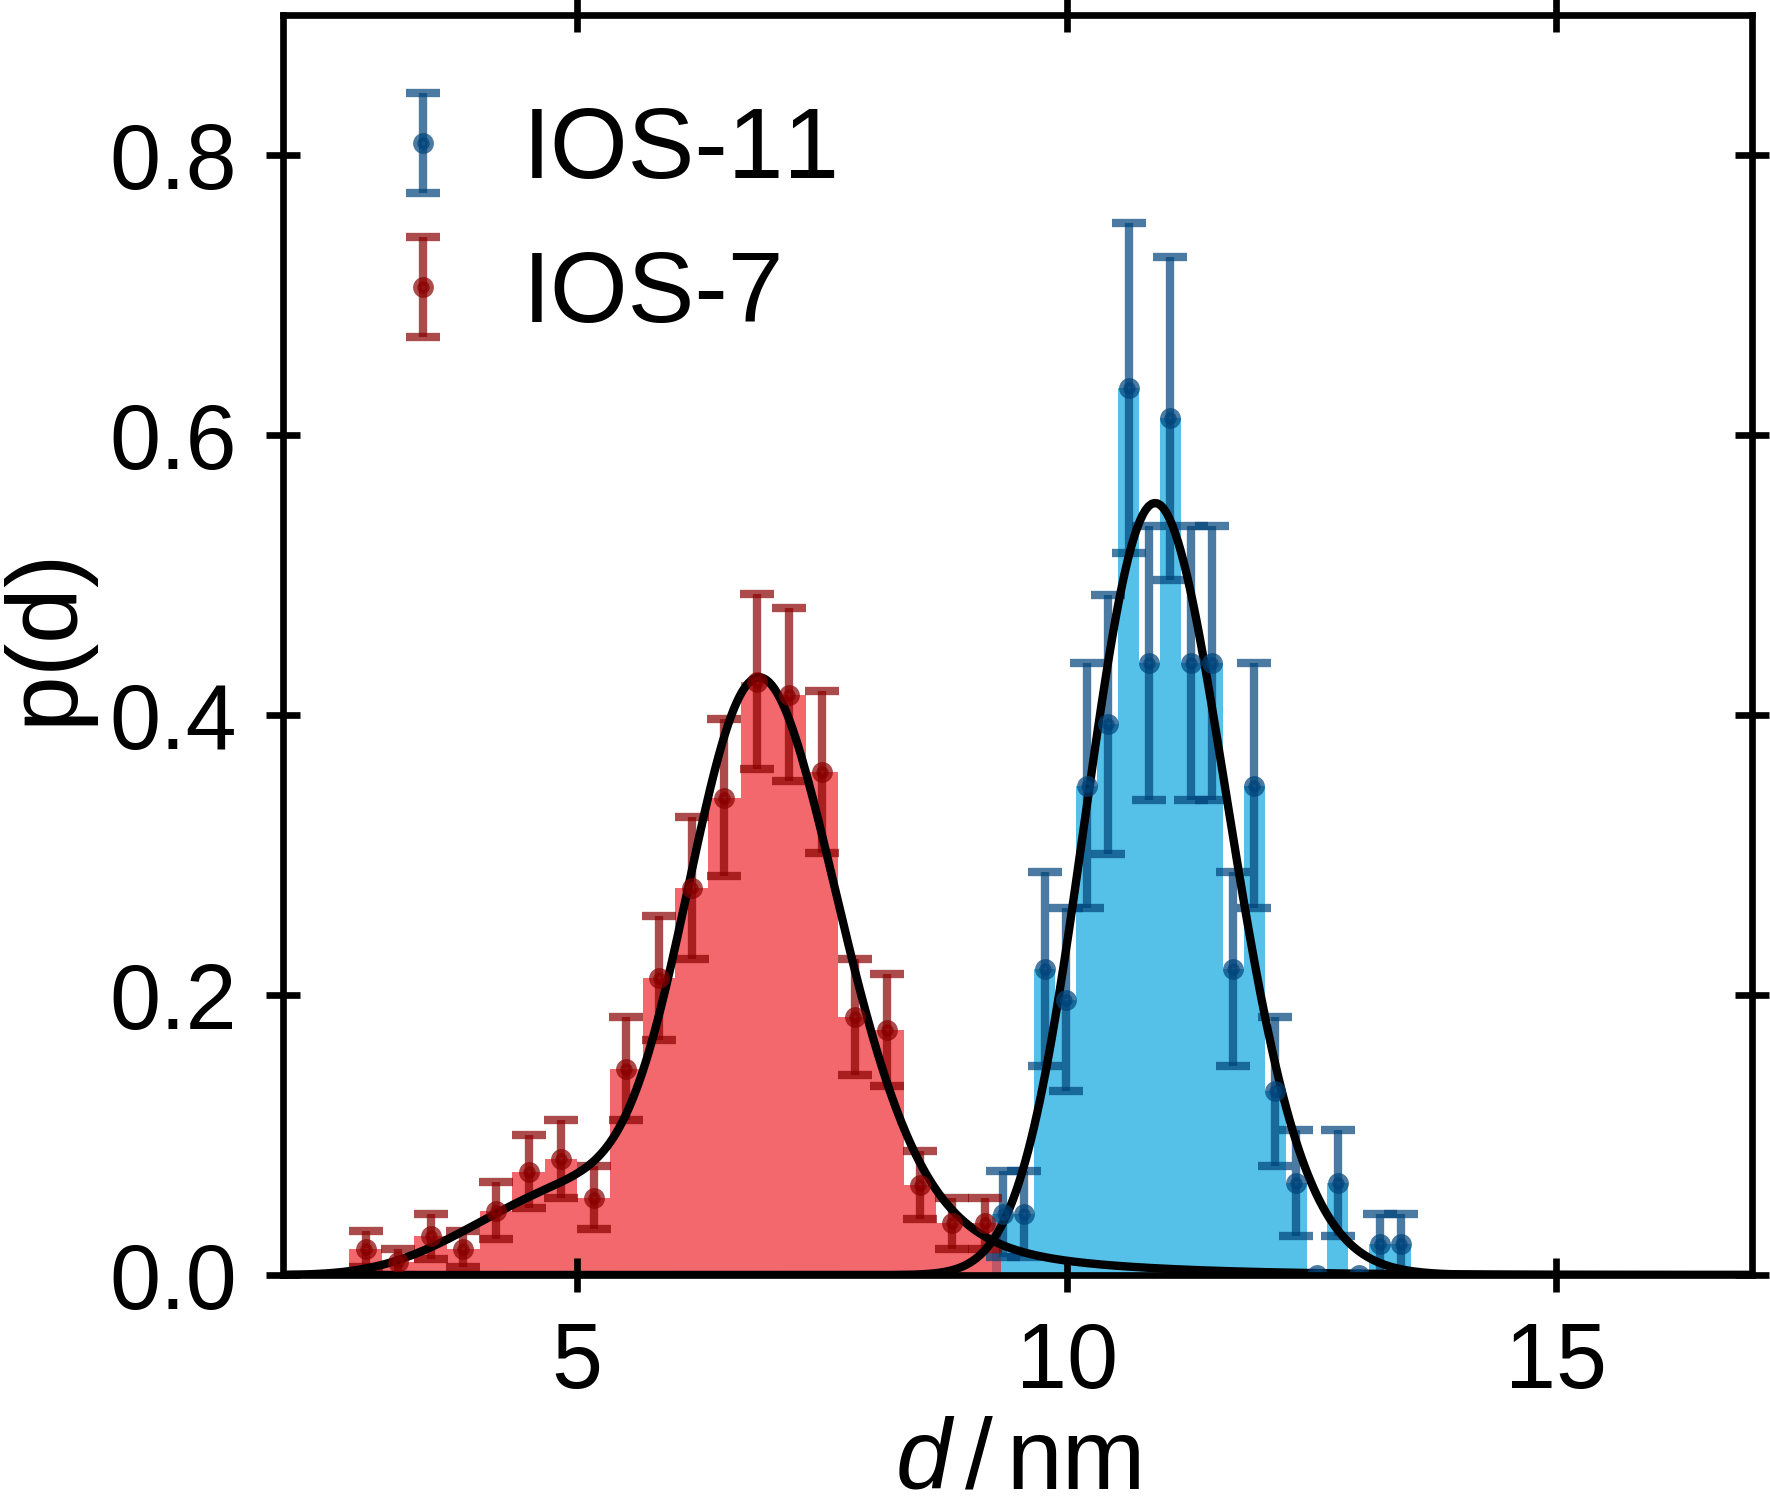
\includegraphics{looselyPackedNP_TEM_PMK18_KWi338_sizeDist}
    \end{minipage}
    \captionof{figure}{\label{fig:looselyPackedNP:nanoparticle:temSizeDist}Size distribution of IOS-7 and IOS-11 extracted from transmission electron microscopy by manually measuring the diameters.}
\end{figure}

Transmission electron microscopy allows to estimate the size from a local snapshot of the dry sample.
A better estimate to quantify the average particle size and size distribution in a dispersion is given by small-angle scattering.
As the particle beam, which has an extension of a few $100 \unitmu$, hits an volume of the dispersion that typically contains $\approx \mathcal{O} (10^{12})$ particles, the estimated parameters from modelling small-angle scattering data is much more representative for the average particle in dispersion than electron microscopy.

Small-angle x-ray scattering (SAXS) experiments were performed on both samples at the \textsc{GALAXI} instrument in the \textsc{Forschungszentrum J\"ulich}, which is described in \refapp{ch:appendix:lss:galaxi}.
Additionally, small-angle neutron scattering (SANS) experiments were performed on the same nanoparticles at the \textsc{D33} instrument at the \textsc{Institute Laue-Langevin} that is described in \refapp{ch:appendix:lss:d33}.
To determine the size of the particles, the data from both experiments is fitted simultaneously to one model.
The particles are modelled as spherical magnetite particles with a brush of oleic acid coated around them.
The particles were dispersed in cyclohexane for the SAXS experiment, and in deuterated toluene for the SANS experiment.
The solvents are chosen to increase the contrast with respect to the oleic acid in the case of SAXS and to minimize the incoherent scattering from hydrogen in the case of SANS.

As in the case of transmission electron microscopy, it is necessary for IOS-7 to add a second mode of particle sizes to obtain a good fit of the data.
The obtained sizes, size distributions are in good agreement to the local result from electron microscopy.


\begin{figure}[tb]
  \centering
  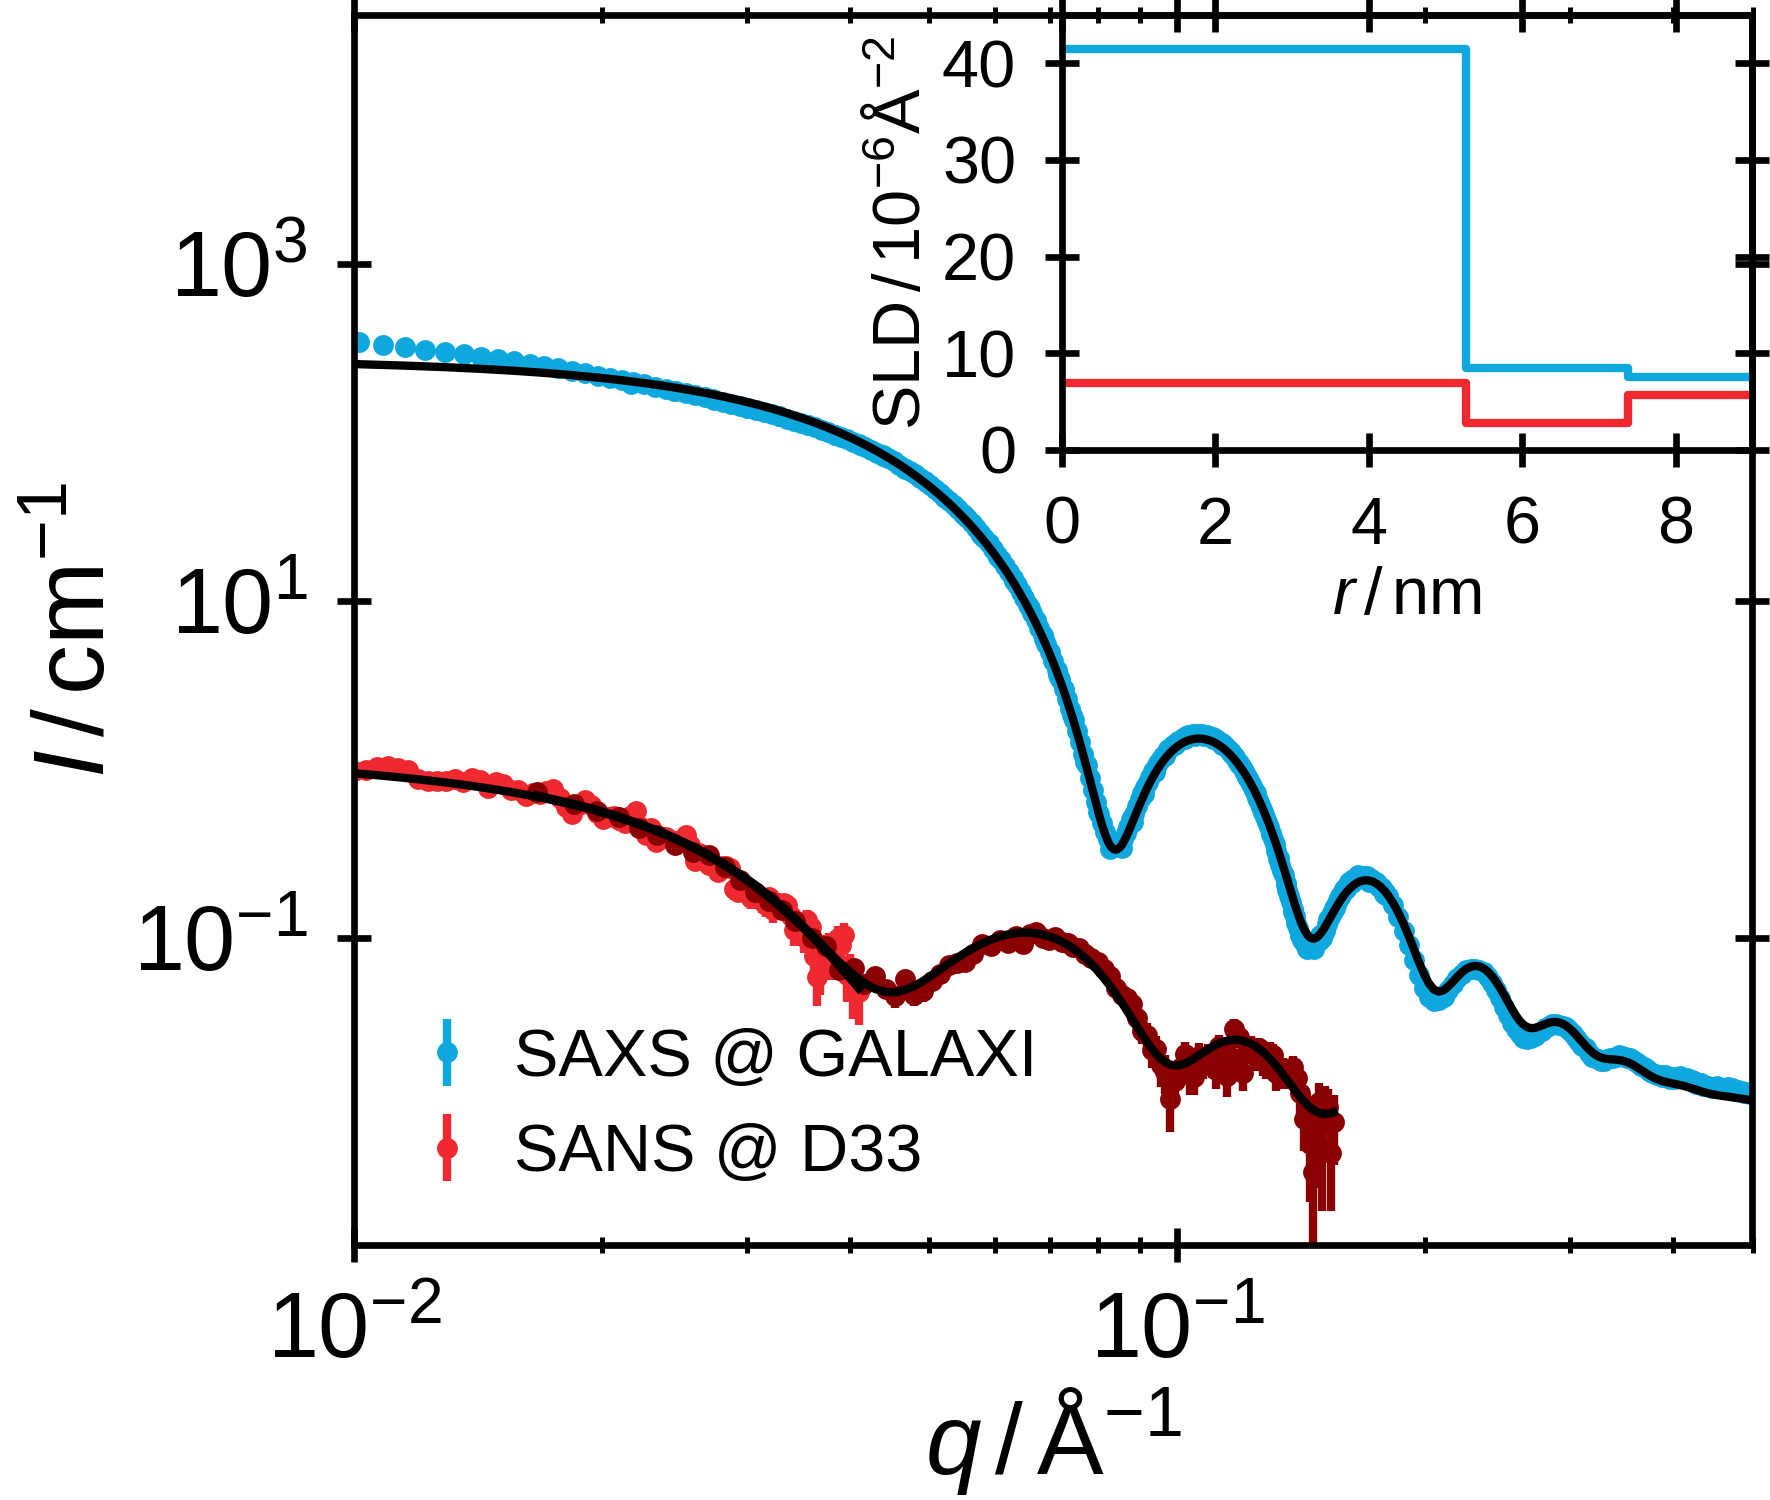
\includegraphics{looselyPackedNP_SAS_IOS-11_SAXSFit}
  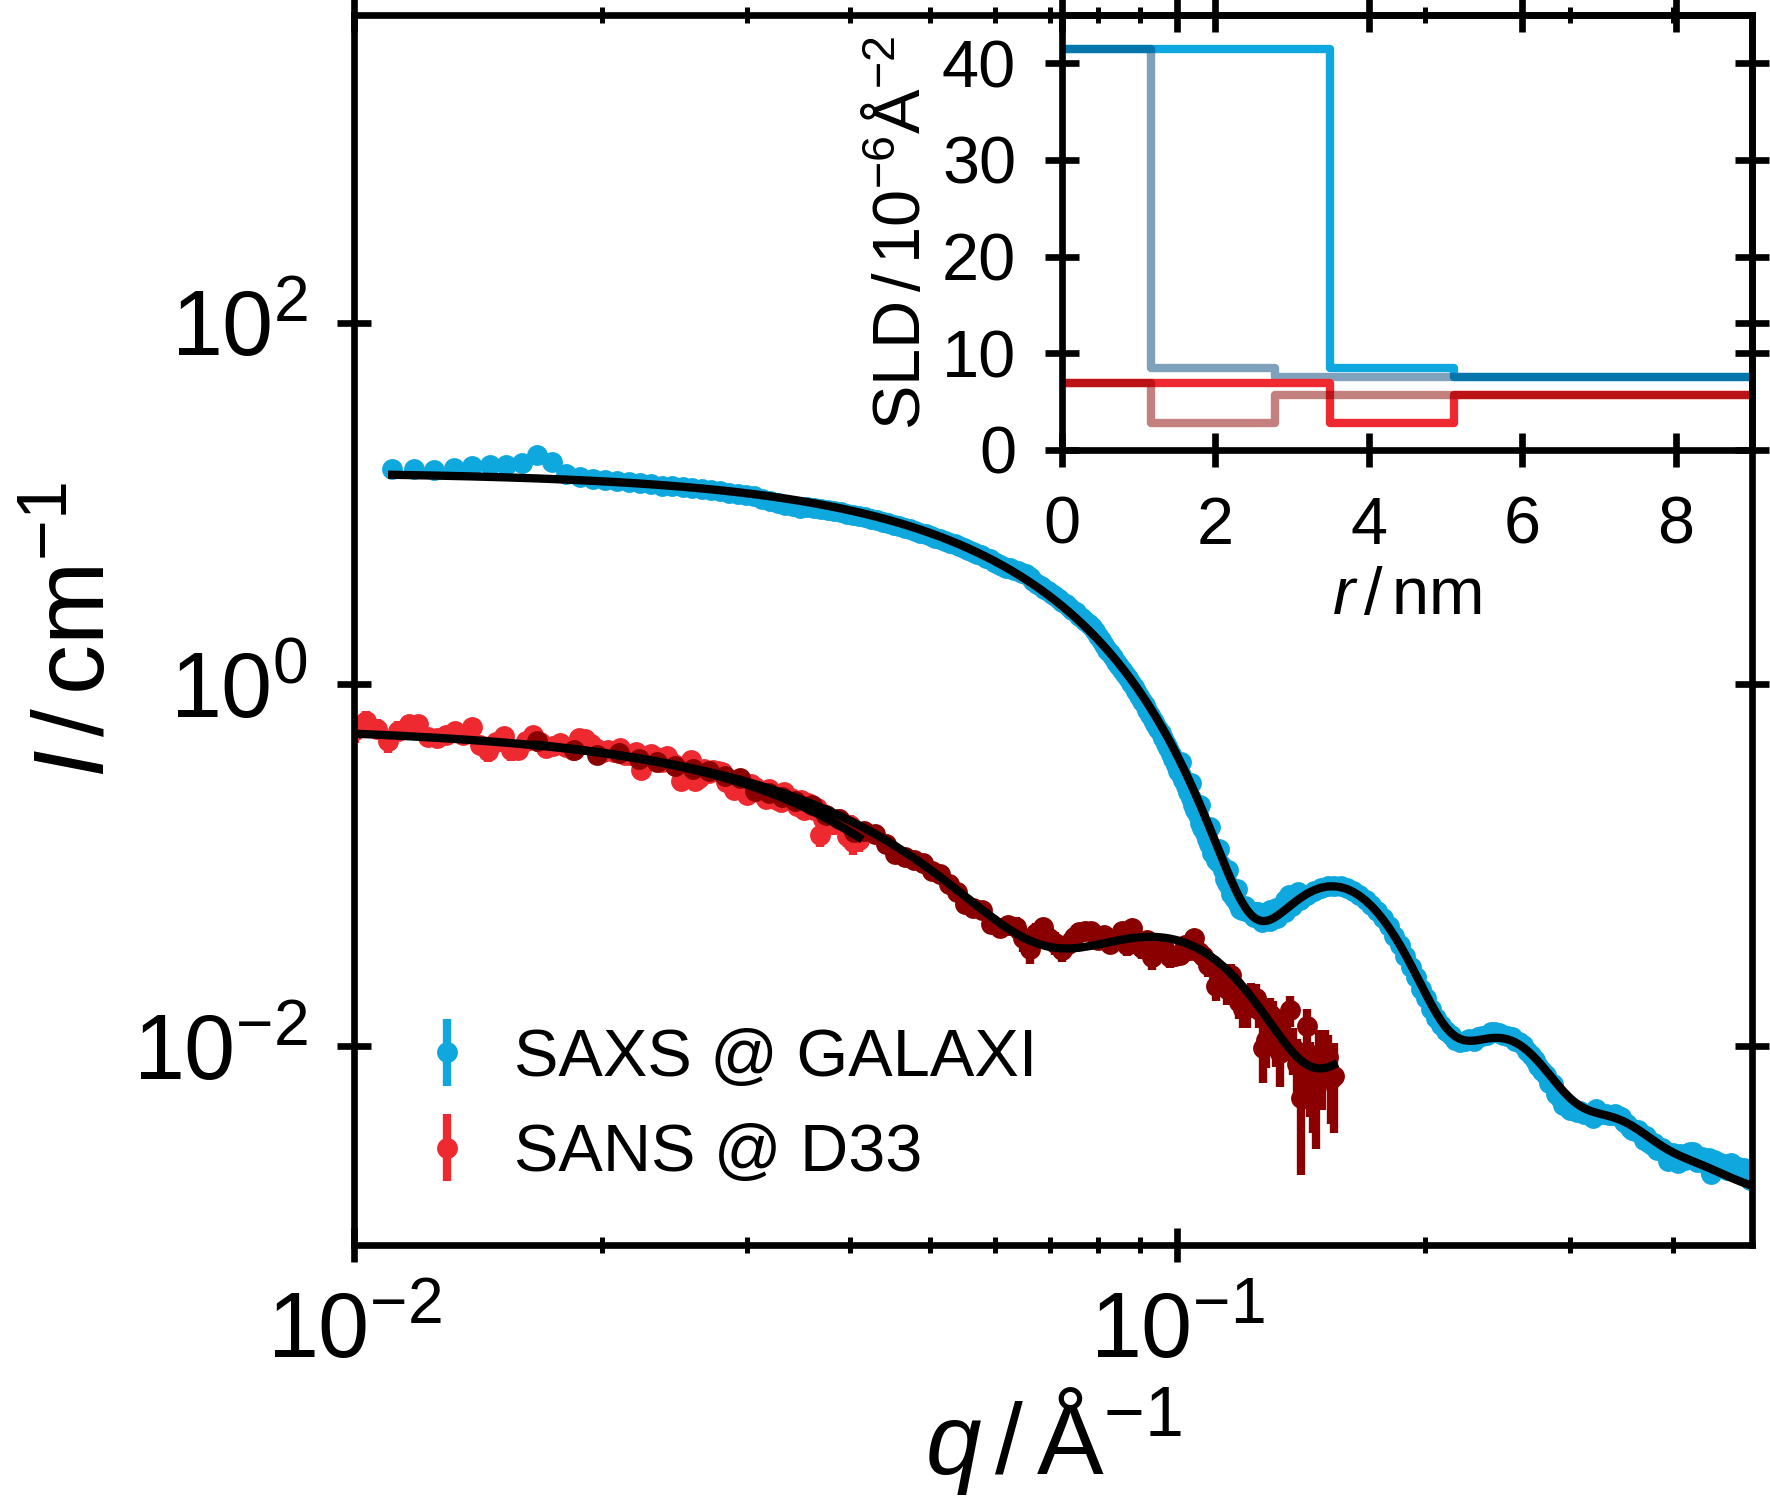
\includegraphics{looselyPackedNP_SAS_IOS-7_SAXSFit}
  \caption{\label{fig:looselyPackedNP:nanoparticle:sas}Small-angle x-ray and neutron scattering for IOS-11 (left) and IOS-7 (right). The x-ray and neutron datasets are fitted simultaneously to a spherical core-shell model to estimate the average size of the particle size and surfactant shell.}
\end{figure}

\begin{table}[tb]
  \centering
  \begin{tabular}{ c | l | l }
      & IOS-11 & IOS-7 \\
    \hline
    $N_1$       & $1$                   & $0.7(1)$   \\
    $\mu_1$     & $10.95(5) \unit{nm}$  & $6.97(6) \unit{nm}$ \\
    $\sigma_1$  & $6.6(4) \unit{\%}$    & $11(1) \unit{\%}$ \\
    $N_2$       & 0                     & $0.3(1)$  \\
    $\mu_2$     & -                     & $6.0(6) \unit{nm}$ \\
    $\sigma_2$  & -                     & $29(4) \unit{\%}$ \\
    \hline
  \end{tabular}
\end{table}
\section{Preparation of Loosely-Packed Layers}

\section{Nuclear Structure}

\section{Magnetic Structure}

\section{Emergent Effects}

\section{Model}

\end{document}